\documentclass{article}

\usepackage{fullpage}
\usepackage{listings}
\usepackage{graphicx}
\usepackage{verbatim}
\usepackage{fancyhdr}

\title{TorFA: Tor Fingerprinting Attack}
\author{Wooyoung Chung -- George Karavaev -- Nathan Dautenhahn}
\date{\today}

\setlength{\headheight}{15.2pt}
\setlength{\headsep}{20pt}

\begin{document}
\maketitle
\setcounter{page}{1}
\newpage
\pagenumbering{roman}
\pagestyle{fancy}
\lhead{Wooyoung Chung -- George Karavaev -- Nathan Dautenhahn}
\chead{}
\rhead{Computer Security II\\Final Report \\ \today}
\tableofcontents 
\listoffigures 
\listoftables 
\newpage
\pagenumbering{arabic}
\setcounter{page}{1}

\section{Introduction}
Online anonymous communication methods are becoming more popular and receiving 
much interest from the research community today. One such method for online 
anonymity is Tor. Tor is a network that provides a method for creating greater 
privacy and security in Internet communications. Tor accomplishes this task 
by using a scheme called onion routing, which uses multiple layers of encryption
and route redirection to provide anonymity to a limited set of web applications 
(e.g. browsing, chat clients). The goal of tor is to disallow an adversary from 
knowing who is requesting and receiving what information on the Internet. 

It has been suggested by the tor developers%\cite{torDoc} 
that Tor could be vulnerable to a website fingerprinting 
attack. In a general fingerprinting attack, an adversary creates a signature of 
a website (based upon what the adversary can view on the network) and builds a 
statistical profile of the website based upon the different characteristics 
of the traffic he can view. This fingerprint is then stored to a fingerprint 
database, which will be used later by the attacker to compare against unknown 
data in order to identify what information a given user is 
viewing. 

This paper introduces a novel method to perform a fingerprinting attack on the 
tor network. TorFA builds a statistical profile on the total number of 
packets downloaded from a given website as the fingerprint data. Then, the 
attacker listens to traffic at the tor entry router, and if the traffic matches 
the pattern of the fingerprint, the attacker knows what web page the client was 
viewing.

%\section{Related Work}

\section{Attack Methodology}
The focus of our attack was to write a set of programs that performed 
two primary tasks: create signatures from a set of known data and compare 
an unknown capture in pcap format to the known set of signatures. The 
second program outputs the best match from the fingerprint database to 
the unknown capture file if such a website exists in the database. 

\subsection{Attack Overview}
The method by which we generated fingerprints was to intercept traffic 
between an entry onion router and the client capturing only traffic that was associated
with the request of a webpage. Once several request and downloads are 
captured the data is processed by an application. This application takes 
as input a directory from which to compute the fingerprint, and several 
other options to allow for specific control of the application. This data
is stored as a file in a fingerprints directory. In this way the fingerprint
``database'' is a directory where each file represents a webpage fingerprint. 

The second application, TorFA, performs the comparison of an unknown webpage 
to the fingerprints in the database. It takes as input a capture of an unknown
webpage (a single stream with only that page's data), which it parses and 
subsequently creates a fingerprint. The application then compares that 
fingerprint to those in the database using K-L divergence. As a result the 
application outputs the best match from the database, if there exists such a match 
(i.e., within $2 *$ Standard Deviation of the total number of packets in the 
known fingerprint). 

\begin{figure}
	\centering
		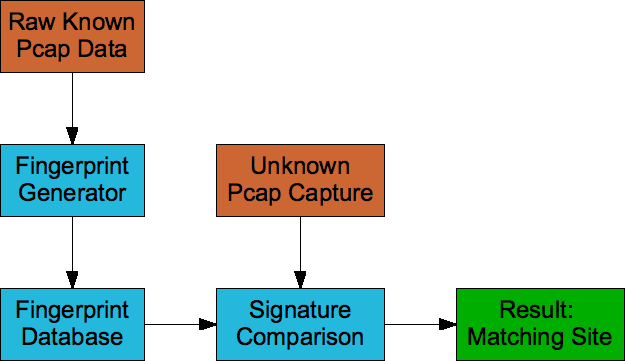
\includegraphics[width=0.5\textwidth]{programFlow.png}
	\caption{Program data and information flow}
	\label{fig:programFlow}
\end{figure}

Figure \ref{fig:programFlow} displays the general flow of information in the 
two applications. Raw known data is sent into the fingerprint creator, 
which outputs a fingerprint into the fingerprint database. Then an unknown
data item is input into the fingerprint comparator, which outputs the 
fingerprint match. 

\subsection{Fingerprint Generation}
The first part of the project included the development of a fingerprinting 
format that could be used for webpage comparisons. Hjelmvik \cite{spid}
showed that probability vectors could be created by using frequency 
analysis of data. TorFA uses this 
same technique in the creation of probability vectors that reflect the unique
data viewable to the attacker. In order to produce such probability vectors
we captured and analyzed website traffic data looking for
patterns that could be used to distinguish one website download from another. 

\subsubsection{Data Collection and Analysis}
Data collection of traffic in a tor flow turns out to be extremely hard to 
accomplish. The first step is defining where to capture the data, which for
this project was chosen to be the client's ethernet port. It was determined
that this was satisfactory because an attacker could view data anywhere along
the route from a client to its associated entry router, and thus without 
loosing any correctness our approach alleviated the need to implement our own 
entry router. 

Collecting data was an arduous task because the tor implementation
does not exactly follow the specification and the encrypted nature of the 
communications protocol. In experiments it was found that tor allows the 
entry routers to choose different port numbers for transferring its TLS data. 
Once this was understood a controlled environment was established to collect
download data using Wireshark. 

Once we had obtained this data we analyzed it for patterns to uniquely identify
a given webpage download. In order to achieve this task a python script was
created to parse and analyze the data for packet counting attributes. The script
uses the command line wireshark equivalent, tshark, to parse the data for useful
information. 

It was determined that the primary attribute of the data was the number of 
packets sent and received from a website of specific size ranges. This is 
intuitive in the sense that a webpage has an approximately fixed size, which 
leads to a similar amount of packets for each download of the webpage. The team
also considered using packet inter-arrival times as an attribute, but due to the
dynamic nature of the tor network an exact time for a webpage download is not 
reproduced on a consistent basis. The analysis here showed one extremely
interesting fact about the tor implementation in that the tor specification
states that all traffic is to be sent in fixed $512$ KB sized frames, but 
in the data we collected packets ranged from $512-4400$ KB size packets. This
turns out to benefit the fingerprint attack because it provides more 
vectors by which the data can be distinguished. 

The end result of the analysis was to use a probability vector that included
packet counts in the size ranges: $0-599$, $600-799$, $800-1449$, and 
$1450-4500$. These ranges were selected because frequency analysis
showed that there were localized packet sizes that dominated the frequency counts, 
and as such the ranges were selected so that each one of these sizes was in a
different range bin. 

\subsection{Fingerprint Comparison}
The method used in this attack to match an unknown fingerprint to a known 
fingerprint is Kullback-Leibler Divergence (K-L divergence). K-L divergence 
is a measure in statistics that quantifies the difference between two 
probability distributions. It is also referred to as relative entropy. The 
following equation is used to measure the difference of a probability 
distribution Q from another probability distribution P: 

\[ D_{KL}(P||Q) = \sum_i P(i)\log\frac{P(i)}{Q(i)}\]

The greater this number is the less Q is like P. In other words, the closer 
the K-L divergence measure is to zero the more accurately Q matches P. In the 
tor fingerprinting attack, P is the probability distribution of the known 
fingerprints, and the distribution Q is a sample of data captured while listing 
to client and entry router communications. 

One shortcoming of this method is that it does not take into consideration 
the potential for a given probability distribution to match another 
distribution and be far off the mean values. E.g., a distribution with packet
counts of $[200,200,200,200]$ will match a distribution with packet counts of
$[1,1,1,1]$. Each one of these counts will produce the same probability 
distribution: $[0.25,0.25,0.25,0.25]$. In order to account for this method 
each probability vector includes 
measures of standard deviation and variance. The standard deviation is used 
to filter out such occurrences thus reducing the false positive rates of the attack.

\section{Adaptive Traffic Shaping: Adding and Dropping}
One method proposed in literature to combat fingerprint attacks is the use 
of traffic shaping mechanisms. These methods include adaptive padding (e.g. 
adding empty packets into a stream) and defensive dropping (e.g. randomly 
dropping good packets) of packets. It is unknown how these methods affect the 
K-L divergence measure of an adversary's attacks in the Tor network. Therefore, 
we modeled a small portion of the Tor network in Mobius, and simulated
traffic shaping methods in order to identify the change in K-L divergence 
measures compared to the costs incurred in the tor network. The costs we 
consider are timing delays experienced by a client request, and the extraneous 
packet increase incurred in the tor network due to the adaptive traffic shaping 
mechanisms. 

The model attempts to simulate a single download of a webpage as captured by 
Wireshark. It provides a simple implementation of the TCP protocol, namely
we have modeled the TCP timeout event and ACK generation. We then model each
entity in a minimal tor network: client, server, entry onion router, middle
onion router, and exit onion router. 

The primary purpose of the model was to quantify the efficacy of adaptive 
traffic techniques 
in terms of the K-L divergence gain verses the cost incurred in the Tor 
network. As such, two models and types of experiments were developed to obtain 
the previously mentioned reward variables. The first set of experiments were 
developed to collect the necessary information for constant add and drop rate
traffic model. The simulation is set up to vary the add and drop packet 
probabilities from 0.0 to 0.3 at .025 length intervals (produces 169 data 
points). In this way, we could 
obtain divergence and cost measurements for multiple combinations of add and 
drop rates. We created a similar study for the variabilistic add and drop 
method which randomly changed this add/drop rate for each new packet as 
opposed to the constant rate for every packet. 

\section{Experimentation}
It is important to note a few aspects of the way that we developed the 
experiments in TorFA. 
\begin{enumerate}
	\item We created the known fingerprints from approximately twenty to 
		thirty samples each. This means that the sample packet counts the 
		produce the probability vector could be bolstered by including several 
		more samples per fingerprint. 
	\item We collected data on two different local host machines. This causes
		great variation in the fingerprints because they differ from one machine
		to the next. To some degree this choice creates a more robust system
		because the victim will be downloading webpages from different machines 
		and host operating systems. 
\end{enumerate}

\section{Results and Analysis}

\subsection{TorFA Results}
\begin{table}[h]
	\centering
		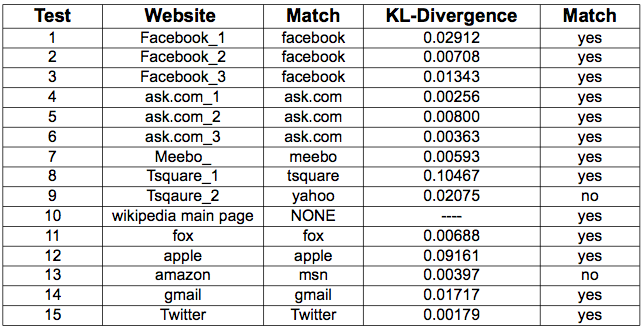
\includegraphics[scale=.6]{../finalpres/results.png}
	\caption{TorFA Results}
	\label{fig:torfaResults}
\end{table}
Table \ref{fig:torfaResults} displays data from the experiments. It show
the test case data and the solution provided by TorFA, and also displays
the divergence measures. As can be seen, most of the websites were detected 
correctly, but this is an extremely small set of sample points.

It is important to recognize that the numbers of K-L divergence in the table 
by themselves are not a complete indicator of how well one sample matched 
against another sample. The estimate cannot give cross correlation between 
the different trials. When looking at 
multiple data output for a given run it can be seen that relatively the K-L
divergence shifts. Meaning that on the smaller K-L divergence measurements
it appears as though most of the measurements for that data run are smaller 
as well.

Another result that is important to recognize is the Wikipedia main website
download. The result for this data point came back as no match because 
this webpage is not in the fingerprint database. This proves to be a successful
trial, but even more than that it shows that even though a webpage might be 
similar to another, for example the Tiananmen Square wikipedia webpage, there
is still enough difference that it will not automatically match. 

\subsection{Adaptive Traffic Shaping}

\subsubsection{Results}
\begin{figure}
	\centering
		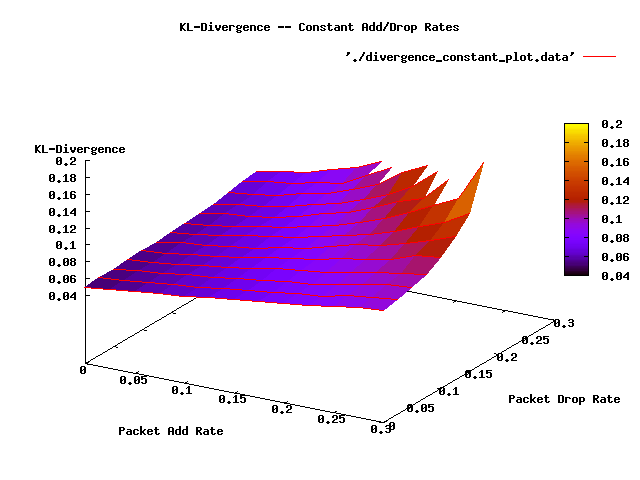
\includegraphics[scale=0.5]{./plots/divergence_constant_plot.png}
	\caption{K-L Divergence Verses Constant Add/Drop Rates}
	\label{fig:divplot}
\end{figure}

\begin{figure}
	\centering
		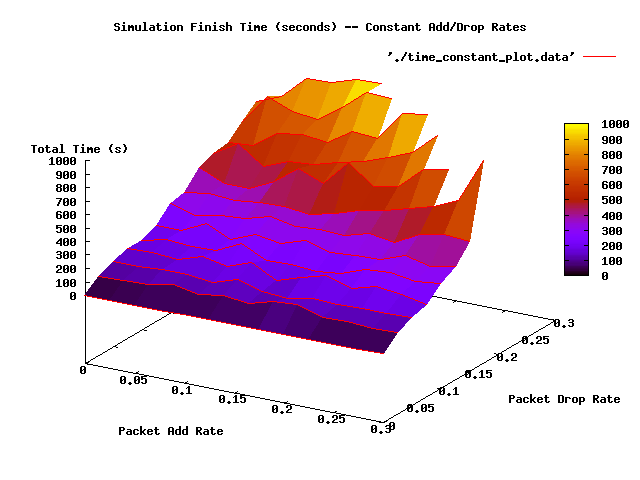
\includegraphics[scale=0.5]{./plots/time_constant_plot.png}
	\caption{Time Verses Constant Add/Drop Rates}
	\label{fig:timeplot}
\end{figure}
\begin{figure}
	\centering
		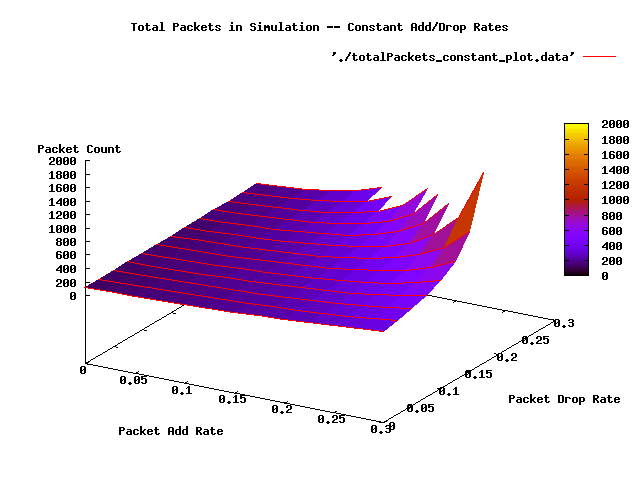
\includegraphics[scale=0.5]{./plots/totalPackets_constant_plot.png}
	\caption{Number of Packets Verses Constant Add/Drop Rates}
	\label{fig:countplot}
\end{figure}
\begin{figure}
	\centering
		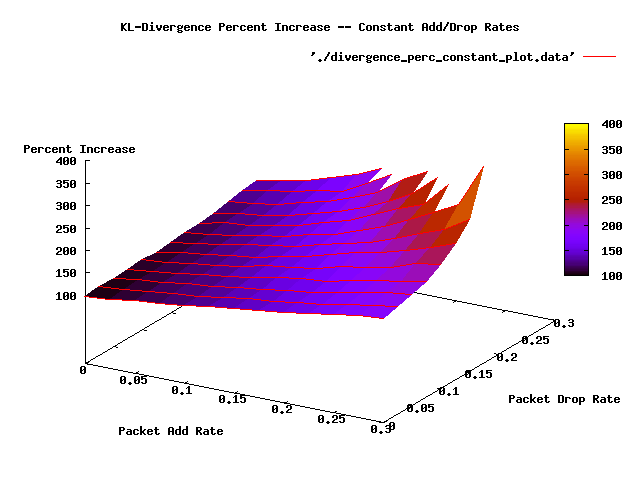
\includegraphics[scale=0.5]{./plots/divergence_perc_constant_plot.png}
	\caption{Percent Increase in the Divergence for Download Simulation}
	\label{fig:divpercplot}
\end{figure}
\begin{figure}
	\centering
		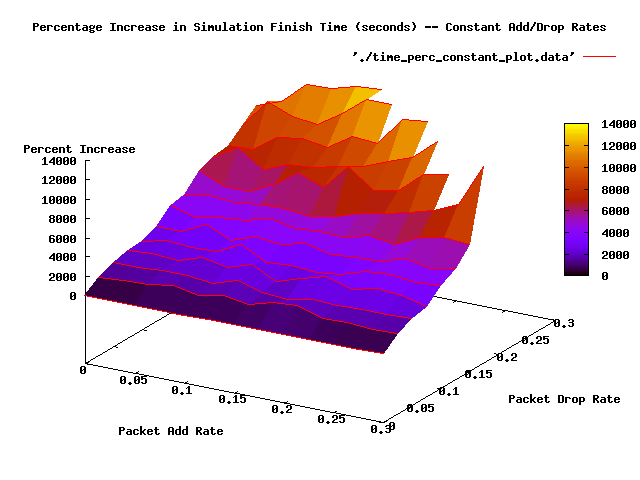
\includegraphics[scale=0.5]{./plots/time_perc_constant_plot.png}
	\caption{Percent Increase in Total Time of Download}
	\label{fig:timepercplot}
\end{figure}
\begin{figure}
	\centering
		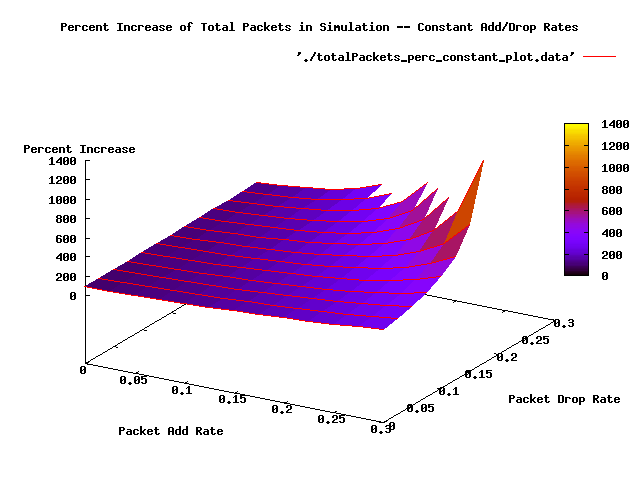
\includegraphics[scale=0.5]{./plots/totalPackets_perc_constant_plot.png}
	\caption{Percent Increase in Total Number of Packets}
	\label{fig:countpercplot}
\end{figure}
\begin{figure}
	\centering
		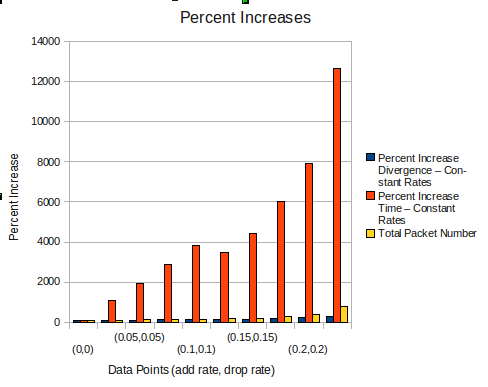
\includegraphics[scale=0.65]{./plots/PercentIncreases_constant.png}
	\caption{Two Dimensional Percent Increase: Divergence, Time, and Total 
		Packets}
	\label{fig:bar1}
\end{figure}
\begin{figure}
	\centering
		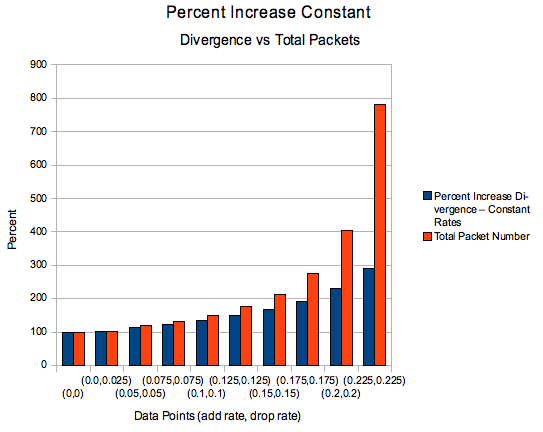
\includegraphics[scale=0.55]{../../code/plots/perc_increase_div_tpacks_constant.png}
	\caption{Two Dimensional Percent Increase: Divergence and Total Packets}
	\label{fig:bar2}
\end{figure}
Figures \ref{fig:divplot}, \ref{fig:timeplot}, and \ref{fig:countplot} 
display the change in divergence at each constant add and drop
packet rate. Figures \ref{fig:divpercplot}, \ref{fig:timepercplot}, and 
\ref{fig:countpercplot} show the percent increase of the labeled data. 
Figures \ref{fig:bar1} and \ref{fig:bar2} show the percent 
increase of the divergence, timing costs, and total transmitted packets in a 
bar chart so that the respective differences can be easily viewed. 

\subsubsection{Analysis}
This data is full of interesting modeling and simulation analysis as well as 
pure fingerprint attack analysis. Some portions of the analysis will be left 
out for brevity's sake.

One important analysis is that the percent increase in total number of packets
displays only the increase in packets for the single download of data as seen
by the attacker. Involved in this data that is missing from the results are 
the added packets that do not make it through the communications channel of the
host to entry router. This is significant because the increase would be much
the same as the time's increase, but even beyond that the tor network would 
become even more congested than these results suggest because the percent
increases here would need to be multiplied by the total number of active 
downloads in the network to correctly model the congestion. 

Another component of these results is that they do not compare the attacker
success rate verses the resultant costs. The divergence gain is two hundred
percent in some cases, but what is not evident is how this affects TorFA. 

\section{Conclusion and Future Work}
The TorFA attack has been shown to be successful at identifying a small 
set of webpage downloads. These results are skewed by the fact that we
do not have a significant amount of data. The next phase of this work will
be to develop automatic methods of performing data capture and processing. In 
this way a large enough sample space can be
evaluated, thus allowing us the surety of statistical tests/methods that
the attack does in fact work. Results such as average success rate, entropy
levels of a given packet size, false-positive/false-negative probabilities, 
and etc. should be obtained so that a high level of confidence can be placed 
in these results. 

The use of adaptive traffic shaping methods increases the KL-divergence 
measurements, but consequently incurs a cost in the form of client request 
timing and extra number of packets in the simulation. The first cost, 
client timing, is negligible because a client could have the extreme 
need for privacy and be willing to wait five to ten minutes to get 
information if it meant that they had a higher probability of being 
undetected. Of course, as this increases very quickly, it may not be useful 
in a practical setting. 

On the other hand the second cost is an extremely important factor because of 
the effect that it has on the rest of the tor network. It is important to note 
that the tor relay routers are provided by users of the system offering up 
their bandwidth and hardware for free. As such, any extra cost to them would 
be a great burden and potentially reduce participation in the network, thus 
reducing the overall privacy of the users in the network, which depends upon 
having a high number of participants to guarantee privacy. This problem is 
further complicated by the fact that our data only includes the extra packets 
that are sent along the fingerprinting attack vector (i.e., the client and 
entry node communication) and not including the internal tor network. These 
added costs would rise similarly to the timing costs and thus be too great of 
a burden upon the tor network. 

Additionally, it can be seen that a KL-divergence increase may not be that 
useful if the attacker's view includes this increase across all of the 
fingerprinted websites. More data collection and analysis are needed in this 
direction in order to quantify the true effects of a KL-divergence increase. 
This would come in the form of a relative measurement and require the explicit 
knowledge of the adversary's attack methodology to quantify accurately. This 
relative measurement is essential for further understanding of the fingerprint 
attack and defenses against it.

A few other future work items include: 
\begin{itemize}
	\item Develop a pcap parser to detect single streams inside a 
		multistreamed data set. The TorFA code currently expects a pcap
		file that is already filtered for one website of traffic. The next
		step in this direction is to research the use of a Fourier transform 
		technique in order to gain some information about individual data 
		streams. This is important because tor multiplexes multiple TCP 
		streams inside of one tor circuit.
	\item Implement the attack as an entry router in the Tor network in order
		 to develop more accurate results. 
	\item As described earlier, more data collection and testing is necessary. 
\end{itemize}

\begin{thebibliography}{9}
	\bibitem{spid}
		Erik Hjelmvik,
		\emph{The SPID Algorithm: Statistical Protocol IDentification}.
		Swedish Internet Infrastructure Foundation, 2008.
\end{thebibliography}

\appendix
%\section{TorFA Code}

%\subsection{Utility Classes}
%\lstinputlisting[language=Python]{../code/FingerprintAttackClasses.py}

%\subsection{Fingerprint Generator}
%\lstinputlisting[language=Python]{../code/createSignature.py}

%\subsection{TorFA Attack}
%\lstinputlisting[language=Python]{../code/torfa.py}
\end{document}
